\documentclass[amsmath, amssymb, aip, jmp, reprint]{revtex4-2}
\usepackage{tikz}
\usetikzlibrary{shapes.geometric}
\usetikzlibrary{decorations.markings}

\begin{document}

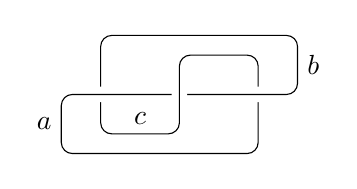
\begin{tikzpicture}[> = latex]

	% Connecting edges

	\draw [draw = white, double = black, double distance between line centers = 3 pt, line width = 2.6 pt, rounded corners](1.5, 0.5) -- (1.5, 0.75) -- (-1, 0.75) -- (-1, -0.5) -- (-0.5, -0.5);
	\draw [draw = white, double = black, double distance between line centers = 3 pt, line width = 2.6 pt, rounded corners] (-1.5, -0.5) -- (-1.5, -0.75) -- (1, -0.75) -- (1, 0.5) -- (0.5, 0.5);
	\draw [draw = white, double = black, double distance between line centers = 3 pt, line width = 2.6 pt, rounded corners] (-1.5, -0.5) -- (-1.5, 0) -- (1.5, 0) -- (1.5, 0.5);
	\draw [draw = white, double = black, double distance between line centers = 3 pt, line width = 2.6 pt, rounded corners] (-0.5, -0.5) -- (0, -0.5) -- (0, 0.5) -- (0.5, 0.5);

	% Quandle elements coloring arcs

	\node [left] at (-1.5, -0.375) {$a$};
	\node [right] at (1.5, 0.375) {$b$};
	\node [above] at (-0.5, -0.5) {$c$}; 

\end{tikzpicture}

\end{document}